\section{What the suite contains}

The suite is organised in groups, each of which targets one kind of defect. Table~\ref{tab:tests} lists them.

\begin{table}[ht]
\centering
\small
\begin{tabularx}{\textwidth}{p{3.4cm}X}
\toprule
Group & What it checks \\
\midrule
Hashes & SHA-1, SHA-256 and HMAC-SHA-256 for the lengths 0, 1, 55, 56, 63, 64, 65, 1000, 32768, 32769, 100000 and 1 MiB, each against the in-kernel result, and with the data sent in several pieces, including key lengths up to the 128 byte limit \\
Hash states & clone and reuse of a session through \code{export}/\code{import} \\
Ciphers & ECB, CBC and CTR with 128, 192 and 256 bit keys for lengths from 16 bytes to 1 MiB, including sizes just under and over 32768 and 100000; encrypt, decrypt roundtrip, and decryption of the board's ciphertext by the reference \\
CTR lengths & 1, 15, 16, 17, 33, 1000, 32769 and 100001 bytes, since CTR accepts any length \\
GCM & several tag lengths, associated data of many lengths including zero, flipped ciphertext bits, a changed header and a forged tag, which must all return \code{EBADMSG} \\
Known answers & published test vectors for hashes and ciphers, to make sure the reference itself is not wrong \\
Error paths & wrong key lengths (1, 15, 17, 20, 31, 33, 64 for the ciphers and GCM) rejected with \code{EINVAL}, valid key lengths accepted, a 128 byte HMAC key accepted, invalid tag lengths rejected, oversized requests \\
Registration & each of the ten driver names is listed in \code{/proc/crypto} with the priority set by the \code{prio} parameter \\
Sysfs & the \code{stats} counters move when work is done, \code{ping} works and rejects malformed input \\
Parameters & results stay correct for different settings of \code{window} and \code{chunk} while the module runs \\
Concurrency & several threads each run a different algorithm at once, and every result is checked \\
Unplug (on demand) & see below \\
\bottomrule
\end{tabularx}
\caption{Groups of checks in the functional suite.}\label{tab:tests}
\end{table}

\section{Choosing a reference}

The test cannot simply ask for \code{cbc(aes)} as its reference, because when the board's algorithms are the only ones registered, or have been given a higher priority, the plain name would resolve to the driver under test. The program therefore builds an explicit software composition, such as \code{cbc(aes-generic)}, trying several names (\code{aes-lib}, \code{aes-generic}, \code{aes-aesni}, \code{aes-arm}) until the kernel accepts one for all three modes. It prints which one it found. For GCM the reference is the generic composition of CTR and GHASH. A test whose reference could depend on the thing it tests would prove nothing.

\section{The unplug test}

\code{tests/afalg\_test unplug} is run on demand because it makes the board vanish for a moment. It needs root. It starts four threads running a mix of operations in a loop, and then:

\begin{enumerate}
  \item waits two seconds and checks that requests succeed and none fail;
  \item \emph{deauthorises} the device through its \code{authorized} file in sysfs, which makes the USB core disconnect it exactly as if the cable were pulled, in the middle of requests;
  \item waits three seconds and checks that requests now fail, and that nothing hangs (an alarm kills the process after 120 seconds, and a hang counts as a failure);
  \item reauthorises the device and waits for the driver to bind again by itself;
  \item checks that requests succeed again.
\end{enumerate}

This is the test of the most dangerous code path, and it needs no one to touch a cable.

\section{Other modes of the test program}

\begin{description}
  \item[\code{bench}] throughput of the main algorithms for 1 MiB, against the local implementation, plus the latency of a 64 byte hash.
  \item[\code{stress [n]}] many streamed hashes of random lengths cut into random pieces, compared with the reference.
  \item[\code{loop <s>}] runs for a given number of seconds, for soak testing.
  \item[\code{sweep}] measures throughput over combinations of \code{window} and \code{chunk}.
\end{description}

\section{Transport only measurements}\label{sec:transport}

The driver's \code{ping} file separates the cost of the USB path and the daemon from the cost of cryptography. The runs below were made on the test machine against the real board, with 200 commands each, and give the throughput each way (data goes to the board and the same amount comes back).

\begin{table}[ht]
\centering
\begin{tabular}{rrrr}
\toprule
Size (bytes) & Window & Time per command ($\mu$s) & Throughput (KB/s) \\
\midrule
64 & 4 & 122 & 510 \\
1024 & 4 & 244 & 4084 \\
4096 & 4 & 684 & 5842 \\
16384 & 4 & 2465 & 6490 \\
32768 & 4 & 4806 & 6658 \\
\bottomrule
\end{tabular}
\caption{Effect of the command size on transport throughput (window 4).}
\end{table}

Small commands are dominated by the fixed cost per command: 122~$\mu$s for 64 bytes. At 32 KiB the transport saturates near 6.5~MB/s. That is the ceiling for any operation on this board, and the cryptographic throughput in the next section lies below it.

\begin{table}[ht]
\centering
\begin{tabular}{rrr}
\toprule
Window & Time per 32 KiB command ($\mu$s) & Throughput (KB/s) \\
\midrule
1 & 8506 & 3761 \\
2 & 5117 & 6252 \\
4 & 4958 & 6453 \\
8 & 4934 & 6484 \\
\bottomrule
\end{tabular}
\caption{Effect of the window on transport throughput (32 KiB commands).}\label{tab:window}
\end{table}

\begin{figure}[ht]
\centering
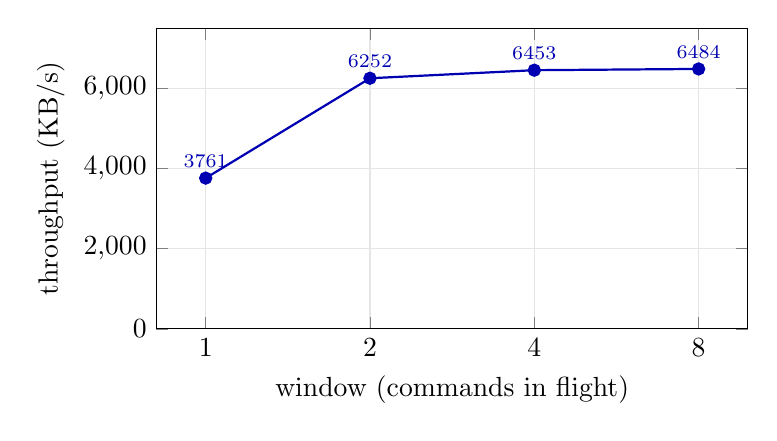
\begin{tikzpicture}
\begin{axis}[
  width=0.75\textwidth,height=5.4cm,
  xlabel={window (commands in flight)},ylabel={throughput (KB/s)},
  xtick={1,2,4,8},xticklabels={1,2,4,8},xmode=log,log basis x=2,
  ymin=0,ymax=7500,grid=both,grid style={black!10},
  every axis plot/.append style={thick},
  nodes near coords,point meta=explicit symbolic,
  nodes near coords style={font=\scriptsize,above}]
\addplot[blue!70!black,mark=*] coordinates {(1,3761)[3761] (2,6252)[6252] (4,6453)[6453] (8,6484)[6484]};
\end{axis}
\end{tikzpicture}
\caption{Measured effect of the window (data of Table~\ref{tab:window}).}
\end{figure}

\paragraph{What the window result shows.} Going from a window of one (stop and wait) to two raises the throughput by about two thirds, because the next command is sent while the board still works on the previous one. A window of four or eight adds almost nothing: with two commands in flight the link is already full. This is the evidence that the design of the command engine does what it was meant to do, and it also shows that the default of four is more than enough for this board. For CBC encryption, which has to run serially, the window cannot help, and the test's throughput for CBC is correspondingly lower.

\section{Cryptographic throughput}

\begin{table}[ht]
\centering
\begin{tabular}{lrr}
\toprule
Operation (1 MiB) & Board (MB/s) & Local CPU (MB/s) \\
\midrule
SHA-256 & 2.79 & 152.84 \\
AES-ECB & 4.22 & \\
AES-CTR & 4.21 & \\
AES-CBC (encrypt) & 2.70 & 180.04 \\
\bottomrule
\end{tabular}
\caption{Throughput from \code{afalg\_test bench}. Local figures vary between runs.}
\end{table}

\paragraph{Reading the numbers.}
\begin{itemize}
  \item ECB and CTR, which can be pipelined, reach about 4.2~MB/s, which is 65 percent of the transport ceiling. The rest of the time is spent in the board's AES engine and in copying.
  \item CBC encryption is about 2.7~MB/s, which is 64 percent of ECB. Each chunk waits for the previous one, so the window gives no benefit, and every chunk pays the full round trip.
  \item SHA-256 is as slow as CBC, 2.8~MB/s. Hashing cannot be split across commands in the same way because each \code{update} depends on the previous state, and the shash interface waits for each reply.
  \item A 64 byte hash takes about 0.62~ms, almost all of it fixed cost per round trip. Demo~5 shows that many concurrent callers can overlap those costs.
  \item The local CPU is roughly 55 to 140 times faster, depending on the run (the local figure was 153 to 394 MB/s in different runs). The project is a demonstration of mechanism.
\end{itemize}
